\chapter{Luyện tập: Từ thông. Cảm ứng điện từ}
\section{Xác định chiều của dòng điện cảm ứng}
\begin{enumerate}
	\item
	{
		Mạch kín tròn (C) nằm trong cùng mặt phẳng P với dòng điện thẳng $I$. Hỏi trường hợp nào dưới đây, từ thông qua (C) biến thiên?
		\begin{center}
			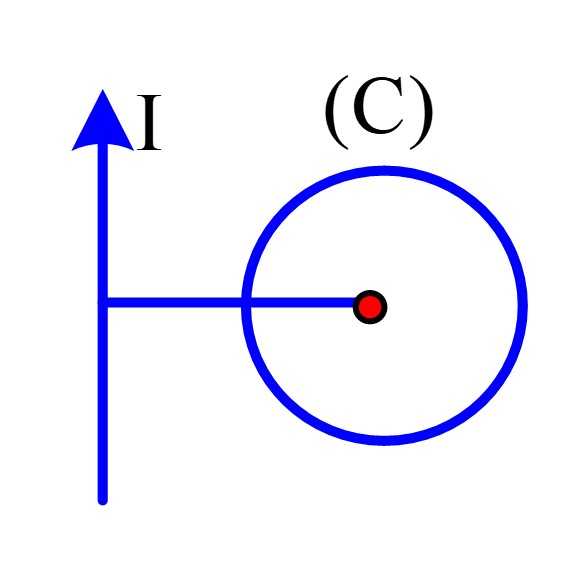
\includegraphics[scale=0.2]{../figs/VN11-PH-29-P-0191-1}
		\end{center}
		\begin{mcq}(1)
			\item{(C) dịch chuyển trong mặt phẳng P lại gần $I$ hoặc ra xa $I$.}
			\item{(C) dịch chuyển trong mặt phẳng P với vận tốc song song với dòng $I$.}
			\item{(C) cố định, dây dẫn thẳng mang dòng $I$ chuyển động tịnh tiến dọc theo chính nó.}
			\item{(C) quay xung quanh dòng điện thẳng $I$.}
		\end{mcq}
	}
	\item
	{
		Cho một nam châm thẳng rơi theo phương thẳng đứng qua tâm $\text O$ của vòng dây dẫn tròn nằm ngang như hình vẽ. Trong quá trình nam châm rơi, vòng dây xuất hiện dòng điện cảm ứng có chiều
		\begin{center}
			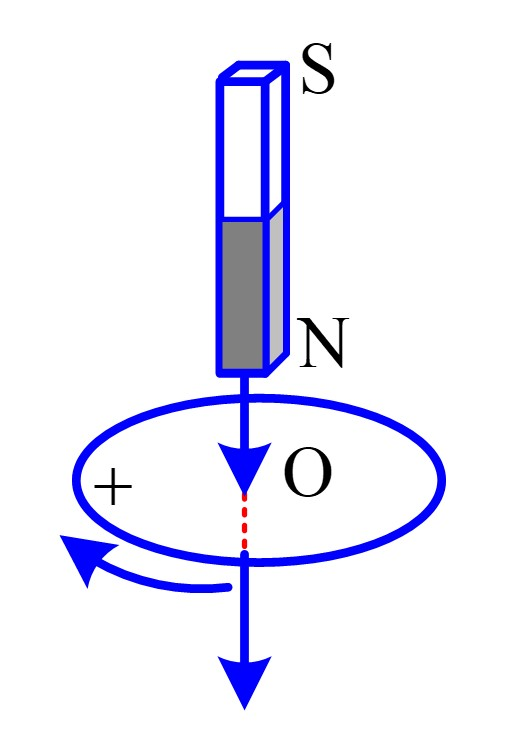
\includegraphics[scale=0.25]{../figs/VN11-PH-29-P-0191-2}
		\end{center}
		\begin{mcq}(1)
			\item{là chiều dương quy ước trên hình.}
			\item{ngược với chiều dương quy ước trên hình.}
			\item{ngược với chiều dương quy ước khi nam châm ở phía trên vòng dây và chiều ngược lại khi nam châm ở phía dưới.}
			\item{là chiều dương quy ước khi nam châm ở phía trên vòng dây và chiều ngược lại khi nam châm ở phía dưới.}
		\end{mcq}
	}
	\item
	{
		Chiều dòng điện cảm ứng trong vòng dây đúng là
		\begin{center}
			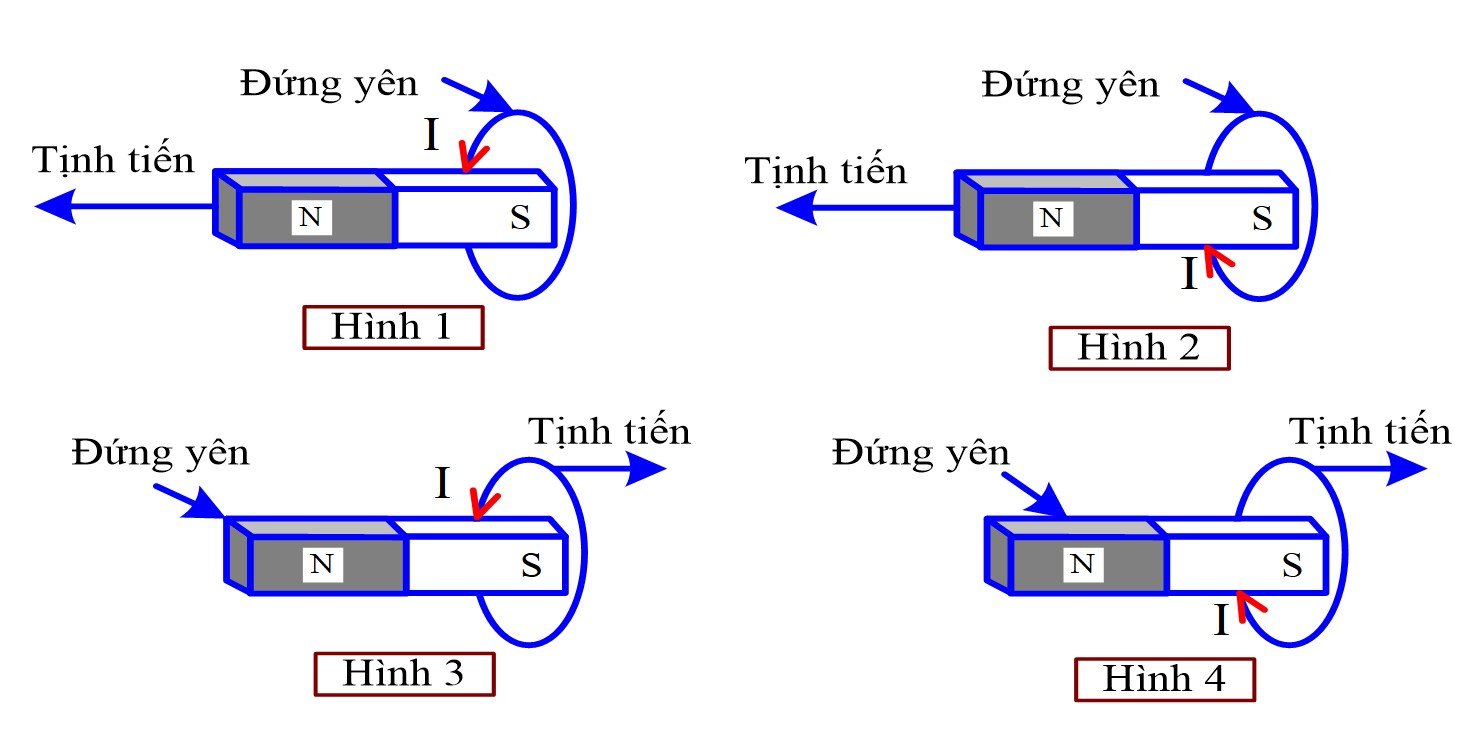
\includegraphics[scale=0.4]{../figs/VN11-PH-29-P-0191-3}
		\end{center}
		\begin{mcq}(2)
			\item{Hình 1 và Hình 2.}
			\item{Hình 1 và Hình 3.}
			\item{Hình 2 và Hình 4.}
			\item{Hình 4 và Hình 3.}
		\end{mcq}
	}
	\item
	{
		Một thanh nam châm NS được đặt thẳng đứng song song với mặt phẳng chứa vòng dây dẫn (C) và có trục quay O vuông góc với trục của vòng dây, chiều dương trên vòng dây được chọn như hình vẽ. Thanh nam châm NS chuyển động quay góc $\ang{90}$ để cực Nam (S) của nó tới đối diện với vòng dây dẫn (C) thì trong (C)
		\begin{center}
			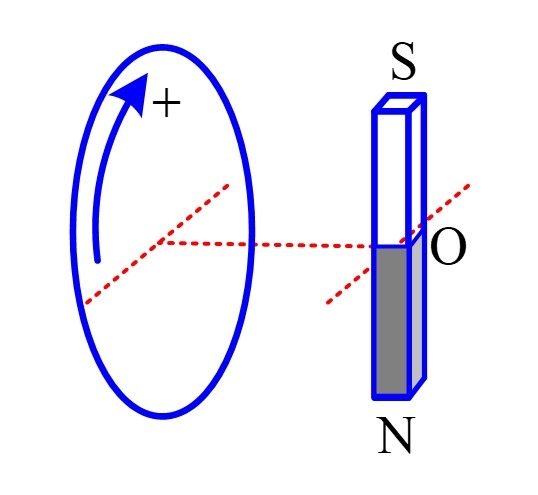
\includegraphics[scale=0.35]{../figs/VN11-PH-29-P-0191-4}
		\end{center}
		\begin{mcq}(1)
			\item{không có dòng điện cảm ứng.}
			\item{có dòng điện cảm ứng chạy theo chiều dương.}
			\item{có dòng điện cảm ứng chạy theo chiều âm.}
			\item{có dòng điện cảm ứng với cường độ biến thiên tuần hoàn theo thời gian.}
		\end{mcq}	
	}
	\item
	{
		Một khung dây dẫn tròn, nhẹ, được treo bằng sợi dây mềm, đường thẳng $x'x$ trùng với trục của khung dây, một nam châm thẳng đặt dọc theo trục $x'x$, cực Bắc của nam châm gần khung dây như hình vẽ. Tịnh tiến nam châm
		\begin{center}
			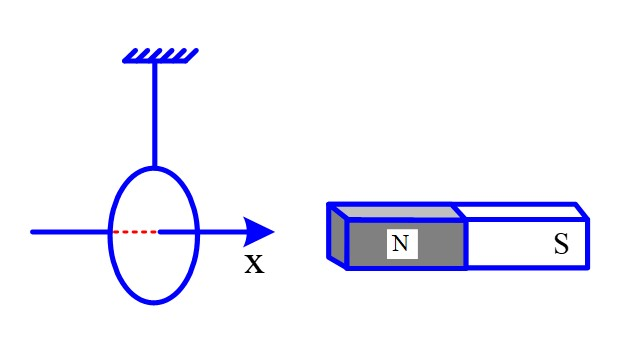
\includegraphics[scale=0.4]{../figs/VN11-PH-29-P-0191-5}
		\end{center}
		\begin{mcq}(1)
			\item{lại gần khung dây thì thấy khung dây chuyển động theo chiều dương trục $x'x$.}
			\item{lại gần khung dây thì thấy khung dây chuyển động theo chiều âm trục $x'x$.}
			\item{ra xa khung dây thì thấy khung dây chuyển động theo chiều âm trục $x'x$.}
			\item{thì chúng luôn đẩy khung dây.}
		\end{mcq}
	}
	\item
	{
		Một khung dây dẫn rất nhẹ được treo bằng sợi dây mềm, đường thẳng $x'x$ trùng với trục của khung dây. Khung dây được đặt gần một nam châm điện, trục nam châm điện trùng với trục $x'x$. Khi cho con chạy của biến trở dịch chuyển từ M đến N thì
		\begin{center}
			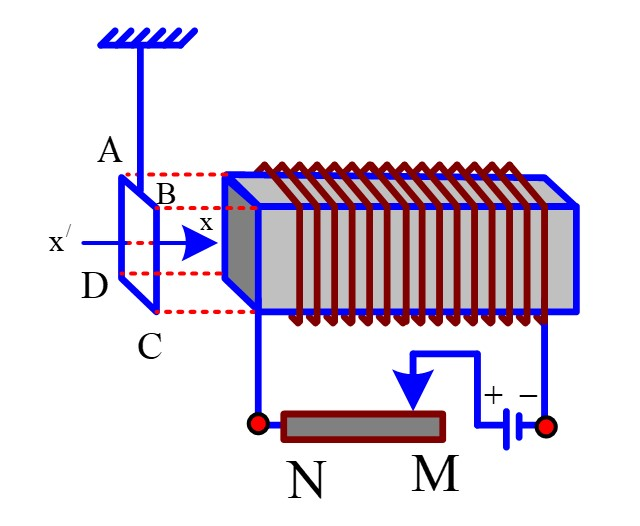
\includegraphics[scale=0.4]{../figs/VN11-PH-29-P-0191-6}
		\end{center}
		\begin{mcq}(1)
			\item{trong khung dây không có dòng điện cảm ứng.}
			\item{trong khung dây xuất hiện dòng điện cảm ứng có chiều ABCD.}
			\item{khung dây bị đẩy ra xa nam châm.}
			\item{khung dây bị hút lại gần nam châm.}
		\end{mcq}	
	}
	\item
	{
		Một khung dây dẫn tròn gồm $N$ vòng. Khung nằm trong từ trường đều, mặt phẳng khung song song với đường sức từ như hình vẽ. Cho khung quay xung quanh trục MN, qua tâm của khung và trùng với một đường sức từ thì
		\begin{center}
			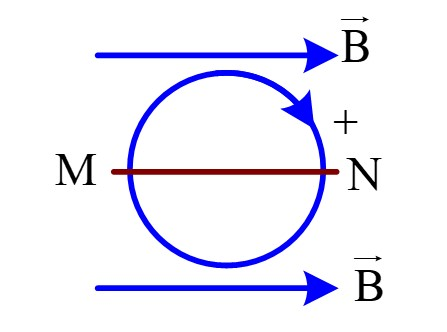
\includegraphics[scale=0.4]{../figs/VN11-PH-29-P-0191-7}
		\end{center}
		\begin{mcq}(1)
			\item{không có dòng điện cảm ứng.}
			\item{có dòng điện cảm ứng chạy theo chiều dương.}
			\item{có dòng điện cảm ứng chạy theo chiều âm.}
			\item{có dòng điện cảm ứng với cường độ biến thiên tuần hoàn theo thời gian.}
		\end{mcq}	
	}
	\item
	{
		Cho dòng điện thẳng cường độ $I$ không đổi và khung dây dẫn hình chữ nhật MNPQ, cạnh MQ của khung sát với dòng điện như hình vẽ. Cho biết các dây dẫn đều có lớp vỏ cách điện. Cho khung dây dẫn quay xung quanh cạnh MQ của khung thì
		\begin{center}
			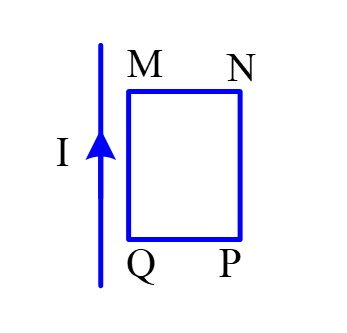
\includegraphics[scale=0.45]{../figs/VN11-PH-29-P-0191-8}
		\end{center}
		\begin{mcq}(1)
			\item{không có dòng điện cảm ứng.}
			\item{có dòng điện cảm ứng chạy theo chiều dương.}
			\item{có dòng điện cảm ứng chạy theo chiều âm.}
			\item{có dòng điện cảm ứng với cường độ biến thiên tuần hoàn theo thời gian.}
		\end{mcq}	
	}
\end{enumerate}
\textbf{Đáp án}
\begin{center}
	\begin{tabular}{|m{2.8em}|m{2.8em}|m{2.8em}|m{2.8em}|m{2.8em}|m{2.8em}|m{2.8em}|m{2.8em}|m{2.8em}|m{2.8em}|}
		\hline
		1. A & 2. C & 3. B & 4. B & 5. B & 6. C & 7. A & 8. A &&\\
		\hline
	\end{tabular}
\end{center}
\section{Bài tập từ thông}
\begin{enumerate}
	\item
	{
		Một vòng dây phẳng giới hạn diện tích $S=\SI{5}{\centi \meter \squared}$ đặt trong từ trường đều cảm ứng từ $B=\SI{0.1}{\tesla}$. Mặt phẳng vòng dây làm thành với từ trường một góc $\alpha = \ang{30}$. Tính từ thông qua $S$.
		\begin{mcq}(4)
			\item{$\SI{3e-4}{\weber}$.}
			\item{$\SI{3e-5}{\weber}$.}
			\item{$\SI{4.5e-5}{\weber}$.}
			\item{$\SI{2.5e-5}{\weber}$.}
		\end{mcq}	
	}
	\item
	{
		Một khung dây hình tròn đặt trong từ trường đều có cảm ứng từ $B=\SI{0.06}{\tesla}$ sao cho mặt phẳng khung dây vuông góc với các đường sức từ. Từ thông qua khung dây là $\SI{1.2e-5}{\weber}$. Bán kính vòng dây gần giá trị nào nhất sau đây?
		\begin{mcq}(4)
			\item{$\SI{12}{\milli \meter}$.}
			\item{$\SI{6}{\milli \meter}$.}
			\item{$\SI{7}{\milli \meter}$.}
			\item{$\SI{8}{\milli \meter}$.}
		\end{mcq}	
	}
	\item
	{
		Một khung dây phẳng giới hạn diện tích $S=\SI{5}{\centi \meter \squared}$ gồm 20 vòng dây đặt trong từ trường đều có cảm ứng từ $B=\SI{0.1}{\tesla}$ sao cho mặt phẳng khung dây hợp với vectơ cảm ứng từ một góc $\ang{60}$. Tính từ thông qua diện tích giới hạn bởi khung dây
		\begin{mcq}(4)
			\item{$\SI{8.66e-4}{\weber}$.}
			\item{$\SI{5e-4}{\weber}$.}
			\item{$\SI{4.5e-5}{\weber}$.}
			\item{$\SI{2.5e-5}{\weber}$.}
		\end{mcq}	
	}
	\item
	{
		Một khung dây hình vuông cạnh $\SI{5}{\centi \meter}$ đặt trong từ trường đều có cảm ứng từ $B=\SI{8e-4}{\tesla}$. Từ thông qua hình vuông đó bằng $\SI{e-6}{\weber}$. Tính góc hợp giữa vectơ cảm ứng từ và vectơ pháp tuyến của hình vuông đó.
		\begin{mcq}(4)
			\item{$\alpha = \ang{0}$.}
			\item{$\alpha=\ang{30}$.}
			\item{$\alpha=\ang{60}$.}
			\item{$\alpha=\ang{90}$.}
		\end{mcq}	
	}
	\item
	{
		[Đề tham khảo của BGD-ĐT-2018] Một khung dây phẳng diện tích $\SI{20}{\centi \meter \squared}$ đặt trong từ trường đều có vectơ cảm ứng từ hợp với vectơ pháp tuyến của mặt phẳng khung dây một góc $\ang{60}$ và có độ lớn $\SI{0.12}{\tesla}$. Từ thông qua khung dây này là
		\begin{mcq}(4)
			\item{$\SI{2.4e-4}{\weber}$.}
			\item{$\SI{1.2e-4}{\weber}$.}
			\item{$\SI{1.2e-6}{\weber}$.}
			\item{$\SI{2.4e-6}{\weber}$.}
		\end{mcq}	
	}
	\textbf{Đáp án}
	\begin{center}
		\begin{tabular}{|m{2.8em}|m{2.8em}|m{2.8em}|m{2.8em}|m{2.8em}|m{2.8em}|m{2.8em}|m{2.8em}|m{2.8em}|m{2.8em}|}
			\hline
			1. D & 2. D & 3. A & 4. C & 5. B &&&&&\\
			\hline
		\end{tabular}
	\end{center}
\end{enumerate}
\section{Bài tập cảm ứng điện từ}
\begin{enumerate}
	\item
	{
		[Đề chính thức của BGD-ĐT-2018] Một vòng dây dẫn kín, phẳng có diện tích $\SI{10}{\centi \meter \squared}$. Vòng dây được đặt trong từ trường đều có vectơ cảm ứng từ hợp với vectơ pháp tuyến của mặt phẳng vòng dây một góc $\ang{60}$ và có độ lớn là $\SI{1.5e-4}{\tesla}$. Từ thông qua vòng dây dẫn này có giá trị là
		\begin{mcq}(4)
			\item{$\SI{1.3e-3}{\weber}$.}
			\item{$\SI{1.3e-7}{\weber}$.}
			\item{$\SI{7.5e-8}{\weber}$.}
			\item{$\SI{7.5e-4}{\weber}$.}
		\end{mcq}	
	}
	\item
	{
		[Đề chính thức của BGD-ĐT-2018] Một vòng dây dẫn kín, phẳng được đặt trong từ trường đều. Trong khoảng thời gian $\SI{0.04}{\second}$, từ thông qua vòng dây giảm đều từ giá trị $\SI{6e-3}{\weber}$ về $0$ thì suất điện động cảm ứng xuất hiện trong vòng dây có độ lớn là
		\begin{mcq}(4)
			\item{$\SI{0.12}{\volt}$.}
			\item{$\SI{0.15}{\volt}$.}
			\item{$\SI{0.30}{\volt}$.}
			\item{$\SI{70.24}{\volt}$.}
		\end{mcq}	
	}
	\item
	{
		Một vòng dây dẫn hình vuông, cạnh $a=\SI{10}{\centi \meter}$, đặt cố định trong một từ trường đều có vectơ cảm ứng từ vuông góc với mặt khung. Trong khoảng thời gian $\SI{0.05}{\second}$, cho độ lớn của cảm ứng từ tăng đều từ $0$ đến $\SI{0.5}{\tesla}$. Xác định độ lớn của suất điện động cảm ứng xuất hiện trong vòng dây
		\begin{mcq}(4)
			\item{$\SI{100}{\volt}$.}
			\item{$\SI{0.1}{\volt}$.}
			\item{$\SI{1.5}{\volt}$.}
			\item{$\SI{0.15}{\volt}$.}
		\end{mcq}	
	}
	\item
	{
		Một khung dây phẳng diện tích $\SI{20}{\centi \meter \squared}$, gồm 10 vòng dây được đặt trong từ trường đều. Vectơ cảm ứng từ làm thành với mặt phẳng khung dây góc $\ang{30}$ và có độ lớn bằng $\SI{2e-4}{\tesla}$. Người ta làm cho từ trường giảm đều đến 0 trong thời gian $\SI{0.01}{\second}$ thì độ lớn suất điện động cảm ứng xuất hiện trong khung dây trong thời gian từ trường biến đổi là
		\begin{mcq}(4)
			\item{$\SI{200}{\micro \volt}$.}
			\item{$\SI{180}{\micro \volt}$.}
			\item{$\SI{160}{\micro \volt}$.}
			\item{$\SI{80}{\micro \volt}$.}
		\end{mcq}	
	}
	\item
	{
		Một khung dây dẫn hình chữ nhật có diện tích $\SI{200}{\centi \meter \squared}$, ban đầu ở vị trí song song với các đường sức từ của một từ trường đều có độ lớn $B=\SI{0.01}{\tesla}$. Khung quay đều trong thời gian $\Delta t= \SI{0.04}{\second}$ đến vị trí vuông góc với các đường sức từ. Độ lớn suất điện động cảm ứng xuất hiện trong khung là
		\begin{mcq}(4)
			\item{$\SI{5}{\milli \volt}$.}
			\item{$\SI{12}{\milli \volt}$.}
			\item{$\SI{3.6}{\volt}$.}
			\item{$\SI{4.8}{\volt}$.}
		\end{mcq}	
	}
	\item
	{
		Một mạch kín hình vuông, cạnh $\SI{10}{\centi \meter}$, đặt vuông góc với một từ trường đều có độ lớn thay đổi theo thời gian. Tính tốc độ biến thiên của cảm ứng từ, biết cường độ dòng điện cảm ứng là $\SI{2}{\ampere}$ và điện trở của mạch là $\SI{5}{\Omega}$.
		\begin{mcq}(4)
			\item{$\SI{1000}{\tesla / \second}$.}
			\item{$\SI{0.1}{\tesla / \second}$.}
			\item{$\SI{1500}{\tesla / \second}$.}
			\item{$\SI{10}{\tesla / \second}$.}
		\end{mcq}	
	}
	\item
	{
		Một ống dây hình trụ dài gồm $1000$ vòng dây, diện tích mỗi vòng dây $S=\SI{100}{\centi \meter \squared}$. Ống dây có điện trở $R=\SI{16}{\Omega}$, hai đầu nối đoản mạch và được đặt trong từ trường đều có vectơ cảm ứng từ song song với trục của ống dây và có độ lớn tăng đều $\SI{e-2}{\tesla / \second}$. Công suất toả nhiệt của ống dây là
		\begin{mcq}(4)
			\item{$\SI{200}{\micro \watt}$.}
			\item{$\SI{680}{\micro \watt}$.}
			\item{$\SI{1000}{\micro \watt}$.}
			\item{$\SI{625}{\micro \watt}$.}
		\end{mcq}	
	}
	\item
	{
		Từ thông qua một khung dây biến thiên theo thời gian được biểu diễn như hình vẽ.
		\begin{center}
			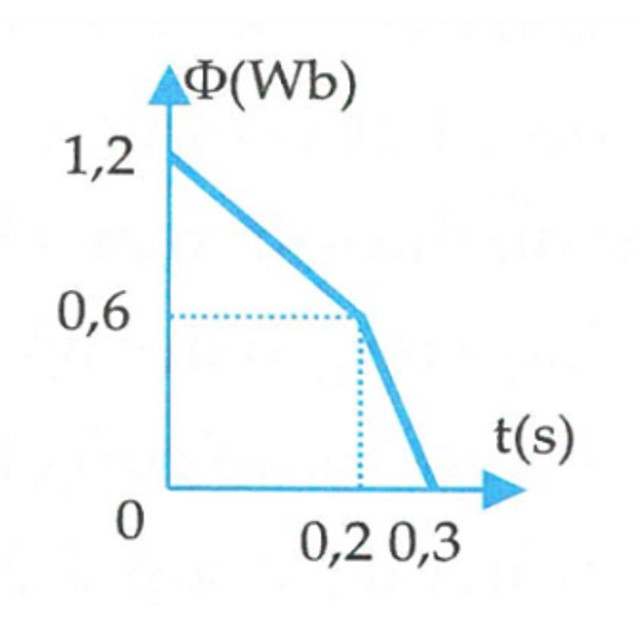
\includegraphics[scale=0.4]{../figs/VN11-PH-29-P-0191-9}
		\end{center}
		Suất điện động cảm ứng trong khung trong các khoảng thời gian tương ứng sẽ là
		\begin{mcq}(1)
			\item{trong khoảng thời gian từ $0$ đến $\SI{0.1}{\second}$: $\varepsilon = \SI{3}{\volt}$.}
			\item{trong khoảng thời gian từ $\SI{0.1}{\second}$ đến $\SI{0.2}{\second}$: $\varepsilon =\SI{6}{\volt}$.}
			\item{trong khoảng thời gian từ $\SI{0.2}{\second}$ đến $\SI{0.3}{\second}$: $\varepsilon =\SI{9}{\volt}$.}
			\item{trong khoảng thời gian từ $0$ đến $\SI{0.3}{\second}$: $\varepsilon =\SI{4}{\volt}$.}
		\end{mcq}	
	}
	\item
	{
		Một khung dây phẳng diện tích $\SI{20}{\centi \meter \squared}$ gồm $100$ vòng đặt trong từ trường đều $B=\SI{2e-4}{\tesla}$, vectơ cảm ứng từ hợp với mặt phẳng khung dây một góc $\ang{30}$. Người ta giảm đều từ trường đến $0$ trong khoảng thời gian $\SI{0.01}{\second}$. Tính suất điện động cảm ứng xuất hiện trong khung trong thời gian từ trường biến đổi.
		\begin{mcq}(4)
			\item{$\SI{e-3}{\volt}$.}
			\item{$\SI{2e-3}{\volt}$.}
			\item{$\SI{3e-3}{\volt}$.}
			\item{$\SI{4e-3}{\volt}$.}
		\end{mcq}	
	}
	\textbf{Đáp án}
	\begin{center}
		\begin{tabular}{|m{2.8em}|m{2.8em}|m{2.8em}|m{2.8em}|m{2.8em}|m{2.8em}|m{2.8em}|m{2.8em}|m{2.8em}|m{2.8em}|}
			\hline
			1. C & 2. B & 3. B & 4. A & 5. A & 6. A & 7. D & 8. A & 9. B &\\
			\hline
		\end{tabular}
	\end{center}
\end{enumerate}